%% 
%% Copyright 2007-2020 Elsevier Ltd
%% 
%% This file is part of the 'Elsarticle Bundle'.
%% ---------------------------------------------
%% 
%% It may be distributed under the conditions of the LaTeX Project Public
%% License, either version 1.2 of this license or (at your option) any
%% later version.  The latest version of this license is in
%%    http://www.latex-project.org/lppl.txt
%% and version 1.2 or later is part of all distributions of LaTeX
%% version 1999/12/01 or later.
%% 
%% The list of all files belonging to the 'Elsarticle Bundle' is
%% given in the file `manifest.txt'.
%% 

%% Template article for Elsevier's document class `elsarticle'
%% with numbered style bibliographic references
%% SP 2008/03/01
%%
%% 
%%
%% $Id: elsarticle-template-num.tex 190 2020-11-23 11:12:32Z rishi $
%%
%%
\documentclass[preprint,12pt]{elsarticle}

%% Use the option review to obtain double line spacing
%% \documentclass[authoryear,preprint,review,12pt]{elsarticle}

%% Use the options 1p,twocolumn; 3p; 3p,twocolumn; 5p; or 5p,twocolumn
%% for a journal layout:
%% \documentclass[final,1p,times]{elsarticle}
%% \documentclass[final,1p,times,twocolumn]{elsarticle}
%% \documentclass[final,3p,times]{elsarticle}
%% \documentclass[final,3p,times,twocolumn]{elsarticle}
%% \documentclass[final,5p,times]{elsarticle}
%% \documentclass[final,5p,times,twocolumn]{elsarticle}

%% For including figures, graphicx.sty has been loaded in
%% elsarticle.cls. If you prefer to use the old commands
%% please give \usepackage{epsfig}

%% The amssymb package provides various useful mathematical symbols
\usepackage{amssymb}
\usepackage{amsmath}
\usepackage{graphicx}
\usepackage{subcaption}
%% The amsthm package provides extended theorem environments
%% \usepackage{amsthm}

%% The lineno packages adds line numbers. Start line numbering with
%% \begin{linenumbers}, end it with \end{linenumbers}. Or switch it on
%% for the whole article with \linenumbers.
%% \usepackage{lineno}

\begin{document}

\begin{frontmatter}

%% Title, authors and addresses

%% use the tnoteref command within \title for footnotes;
%% use the tnotetext command for theassociated footnote;
%% use the fnref command within \author or \address for footnotes;
%% use the fntext command for theassociated footnote;
%% use the corref command within \author for corresponding author footnotes;
%% use the cortext command for theassociated footnote;
%% use the ead command for the email address,
%% and the form \ead[url] for the home page:
%% \title{Title\tnoteref{label1}}
%% \tnotetext[label1]{}
%% \author{Name\corref{cor1}\fnref{label2}}
%% \ead{email address}
%% \ead[url]{home page}
%% \fntext[label2]{}
%% \cortext[cor1]{}
%% \affiliation{organization={},
%%             addressline={},
%%             city={},
%%             postcode={},
%%             state={},
%%             country={}}
%% \fntext[label3]{}


\title{Kullback-Leibler Divergence: A Statistical Bridge Between Information Theory and Machine Learning}

%% use optional labels to link authors explicitly to addresses:
%% \author[label1,label2]{}
%% \affiliation[label1]{organization={},
%%             addressline={},
%%             city={},
%%             postcode={},
%%             state={},
%%             country={}}
%%
%% \affiliation[label2]{organization={},
%%             addressline={},
%%             city={},
%%             postcode={},
%%             state={},
%%             country={}}

\author[inst1]{[Sivakumar Ramakrishnan]}
\affiliation[inst1]{organization={Department of Data Science},
            addressline={University of Colorado Boulder}, 
            city={Boulder},
            state={Colorado},
            country={US}}


\author[inst2]{[Sai Nandini Tata]}
\affiliation[inst2]{organization={Department of Data Science},
            addressline={University of Colorado Boulder}, 
            city={Boulder},
            state={Colorado},
            country={US}}

\author[inst3]{[Deep Shukla]}
\affiliation[inst3]{organization={Department of Data Science},
            addressline={University of Colorado Boulder}, 
            city={Boulder},
            state={Colorado},
            country={US}}


\begin{abstract}
This paper provides an empirical investigation of Kullback-Leibler (KL) divergence through the lens of binary classification using machine learning algorithms and deep learning. We first establish the theoretical foundations of KL divergence and its role in machine learning. Through a series of experiments with three different classification models, we visualize and analyze how the KL divergence evolves during the training process and influences the behavior of the model. We show how finding maximum likelihood is the same as minimizing KL divergence loss. Additionally, we explore the application of KL divergence in Variational Autoencoders (VAEs), demonstrating its crucial role in latent space regularization. Our analysis provides insights into both the theoretical and practical aspects of KL divergence in modern machine learning applications.
\end{abstract}

\begin{keyword}
Kullback-Leibler divergence \sep binary classification \sep variational autoencoder \sep deep learning \sep information theory \sep model training dynamics \sep Maximum likelihood estimation
\end{keyword}


\end{frontmatter}

%% \linenumbers

%% main text
\section{Introduction}

\subsection{Background and Motivation}
The Kullback-Leibler (KL) divergence, also known as relative entropy, is one of the most fundamental concepts bridging information theory and statistical inference. Originally introduced by Solomon Kullback and Richard Leibler in 1951, this measure has become increasingly relevant in modern statistical applications, particularly in machine learning and Bayesian inference. In its essence, KL divergence quantifies the difference between two probability distributions on the same random variable. Unlike traditional metrics, it is not symmetric and does not satisfy the triangle inequality, yet these very properties make it uniquely suited for many statistical applications. While its mathematical properties are well-understood, visualizing and understanding its behavior during model training can provide valuable insights into learning dynamics and model optimization.

\subsection{Research Objectives}
This paper aims to:
\begin{itemize}
    \item Visualize and analyze the evolution of KL divergence during the training of three different binary classification models
    \item Compare how different model architectures affect the behavior of KL divergence
    \item Demonstrate the role of KL divergence in Variational Autoencoders
    \item Provide practical insights into the relationship between KL divergence and model performance
\end{itemize}

\section{Theoretical Framework}
\subsection{Connection to Maximum Likelihood Estimation}
The connection between KL divergence and maximum likelihood estimation (MLE) provides a theoretical foundation for many machine learning objectives. Consider a parametric model $q_\theta(x)$ trying to approximate the true data distribution $p(x)$. The MLE objective is to maximize:

$
\mathcal{L}(\theta) = \mathbb{E}_{x \sim p(x)}[\log q_\theta(x)]
$

This is equivalent to minimizing:

$
-\mathcal{L}(\theta) = -\mathbb{E}_{x \sim p(x)}[\log q_\theta(x)]
= \mathbb{E}_{x \sim p(x)}[-\log q_\theta(x)]
$

The KL divergence between the true distribution $p(x)$ and our model $q_\theta(x)$ is:

$
D_{KL}(p||q_\theta) = \mathbb{E}_{x \sim p(x)}\left[\log \frac{p(x)}{q_\theta(x)}\right]
= \mathbb{E}_{x \sim p(x)}[\log p(x)] - \mathbb{E}_{x \sim p(x)}[\log q_\theta(x)]
$

Note that the first term is independent of $\theta$. Therefore, minimizing KL divergence is equivalent to maximizing the expected log-likelihood:

$
\arg\min_\theta D_{KL}(p||q_\theta) = \arg\max_\theta \mathbb{E}_{x \sim p(x)}[\log q_\theta(x)]
$

This equivalence explains why many probabilistic models trained with maximum likelihood can be interpreted as minimizing the KL divergence between the empirical data distribution and the model distribution. This connection is particularly important because:

\begin{itemize}
    \item It provides a theoretical justification for using maximum likelihood estimation
    \item It helps explain the behavior of learned models under different loss functions
    \item It guides the choice of model architectures and training objectives in modern deep learning
\end{itemize}
\subsection{Relationship between KL Divergence and Cross-Entropy}
The relationship between KL divergence and cross-entropy is fundamental to understanding why cross-entropy is commonly used as a loss function in machine learning. Consider two probability distributions $P$ and $Q$. The KL divergence can be expressed as:

$
D_{KL}(P||Q) = \sum_{x} P(x) \log \left(\frac{P(x)}{Q(x)}\right)
= \sum_{x} P(x) \log P(x) - \sum_{x} P(x) \log Q(x)
= -H(P) + H(P,Q)
$

where $H(P)$ is the entropy of distribution $P$, and $H(P,Q)$ is the cross-entropy between $P$ and $Q$. This decomposition reveals that:

$
H(P,Q) = H(P) + D_{KL}(P||Q)
$

When training a machine learning model, $P$ represents the true data distribution and is fixed. Therefore, $H(P)$ is constant with respect to our model parameters. Since KL divergence is non-negative, minimizing cross-entropy is equivalent to minimizing KL divergence. Cross-entropy is preferred in practice because:

\begin{itemize}
    \item It has a simpler computational form that avoids computing $P(x)\log P(x)$ terms
    \item It directly connects to information theory principles of optimal coding
    \item It often leads to more stable numerical computations in practice
\end{itemize}



\subsection{Mathematical Foundations of KL Divergence}
The Kullback-Leibler (KL) divergence, also known as relative entropy, is a measure of the difference between two probability distributions $P$ and $Q$ defined over the same probability space. For discrete probability distributions, the KL divergence is defined as:

$
D_{KL}(P||Q) = \sum_{x \in \mathcal{X}} P(x) \log \left(\frac{P(x)}{Q(x)}\right)
$

For continuous probability distributions, it takes the form of an integral:

$
D_{KL}(P||Q) = \int_{-\infty}^{\infty} p(x) \log \left(\frac{p(x)}{q(x)}\right) dx
$

where $p(x)$ and $q(x)$ are the probability density functions of $P$ and $Q$ respectively.

\subsubsection{Key Properties}
\begin{enumerate}
    \item \textbf{Non-negativity}: $D_{KL}(P||Q) \geq 0$ for all distributions $P$ and $Q$, with equality if and only if $P = Q$ almost everywhere.
    
    \item \textbf{Asymmetry}: Generally, $D_{KL}(P||Q) \neq D_{KL}(Q||P)$, making it not a true metric.
    
    \item \textbf{Chain Rule}: For joint distributions, KL divergence satisfies:
    $D_{KL}(P(X,Y)||Q(X,Y)) = D_{KL}(P(X)||Q(X)) + D_{KL}(P(Y|X)||Q(Y|X))$
\end{enumerate}

\subsection{KL Divergence in Binary Classification}
In binary classification, KL divergence forms the theoretical foundation of the commonly used cross-entropy loss function. Consider a binary classification problem where:
\begin{itemize}
    \item $P(x)$ represents the true label distribution (0 or 1)
    \item $Q(x)$ represents the model's predicted probability distribution
\end{itemize}

The relationship between cross-entropy loss and KL divergence can be expressed as:

$
H(P,Q) = -\sum_{x} P(x) \log Q(x) = H(P) + D_{KL}(P||Q)
$

where $H(P)$ is the entropy of the true distribution $P$. Since $H(P)$ is constant with respect to our model's predictions, minimizing cross-entropy loss is equivalent to minimizing the KL divergence between $P$ and $Q$.

\subsubsection{Training Dynamics}
During model training, the KL divergence serves as a measure of how well our model's predicted probabilities align with the true distribution. For a single binary classification example:

$
D_{KL}(P||Q) = p_1 \log \left(\frac{p_1}{q_1}\right) + (1-p_1) \log \left(\frac{1-p_1}{1-q_1}\right)
$

where $p_1$ is the true probability (usually 0 or 1) and $q_1$ is the model's predicted probability.

\subsection{Role in Variational Autoencoders}
In Variational Autoencoders (VAEs), KL divergence plays a crucial role in the regularization of the latent space. The VAE loss function consists of two terms:

$
\mathcal{L}(\theta, \phi) = \mathbb{E}_{q_\phi(z|x)}[\log p_\theta(x|z)] - D_{KL}(q_\phi(z|x)||p(z))
$

where:
\begin{itemize}
    \item $q_\phi(z|x)$ is the encoder's approximation of the posterior
    \item $p(z)$ is the prior distribution (usually $\mathcal{N}(0,I)$)
    \item $p_\theta(x|z)$ is the decoder's likelihood function
\end{itemize}

The KL divergence term encourages the learned latent distribution to be similar to the prior distribution, preventing the model from learning a degenerate latent representation. For Gaussian distributions, this term has a closed form:

$
D_{KL}(\mathcal{N}(\mu, \sigma^2)||\mathcal{N}(0,1)) = \frac{1}{2}(\mu^2 + \sigma^2 - \log(\sigma^2) - 1)
$

This formulation enables efficient optimization while maintaining the probabilistic interpretation of the latent space.

\section{Experimental Setup}
\subsection{Datasets}
Our experiments utilize three distinct datasets to comprehensively evaluate the behavior of KL divergence across different machine learning tasks and architectures:

\subsubsection{Lung Cancer Dataset}
The lung cancer dataset comprises medical records with 15 features including patient demographics (gender, age) and various symptoms (smoking, anxiety, fatigue, etc.). The binary classification task involves predicting lung cancer presence (positive/negative). The dataset contains balanced classes, making it suitable for evaluating probabilistic predictions. We preprocessed the categorical variables using one-hot encoding and standardized numerical features to zero mean and unit variance.

\subsubsection{Spam Classification Dataset}
For text classification, we employed a ham/spam email dataset to analyze how KL divergence behaves in natural language processing tasks. The dataset consists of email text and binary labels (spam/non-spam). We preprocessed the text using TF-IDF vectorization with a maximum of 1,000 features, capturing the most relevant terms while maintaining computational efficiency.

\subsubsection{MNIST Dataset}
To study KL divergence in the context of deep generative models, we used the MNIST dataset of handwritten digits. This well-established dataset contains 60,000 training images and 10,000 test images, each being 28×28 grayscale pixels. The images were normalized to [0,1] range before training.

\subsubsection{Abalone Dataset}
We also utilized the abalone dataset for binary classification, converting the 'Type' feature into a binary target (M vs. non-M). The dataset includes physical measurements such as shell length, diameter, height, and various weight measurements. This provided a concrete example for visualizing the convergence of maximum likelihood estimation and KL divergence minimization.


\subsection{Model Architectures}
We implemented multiple model architectures to compare how different approaches affect the distribution matching process:

\subsubsection{Binary Classification Models}
For the lung cancer prediction task, we implemented three distinct architectures:
\begin{itemize}
    \item \textbf{Logistic Regression}: A linear model serving as our baseline, using L2 regularization and optimized with stochastic gradient descent.
    
    \item \textbf{Random Forest}: An ensemble model with 100 trees, providing non-linear decision boundaries and naturally bounded probability estimates.
    
    \item \textbf{Neural Network}: A three-layer architecture (input → 64 → 32 → 1) with ReLU activations and dropout (0.3) for regularization, culminating in a sigmoid output layer for probability estimation.
\end{itemize}

\subsubsection{Spam Classification Model}
For text classification, we employed a neural network architecture specifically designed for high-dimensional sparse input:
\begin{itemize}
    \item Input layer matching TF-IDF dimensionality (1,000)
    \item Two hidden layers (128 and 64 units) with ReLU activation
    \item Dropout layers (0.3) for regularization
    \item Sigmoid output layer for binary classification
\end{itemize}

\subsubsection{Variational Autoencoder}
For the MNIST dataset, we implemented a VAE with the following structure:
\begin{itemize}
    \item \textbf{Encoder}: Two fully connected layers (784 → 400 → 400) with ReLU activation
    \item \textbf{Latent Space}: 2-dimensional representation with separate networks for mean and log-variance estimation
    \item \textbf{Decoder}: Mirror of the encoder architecture (2 → 400 → 400 → 784) with sigmoid output activation
\end{itemize}

\subsection{Training Protocol}
All models were trained using the Adam optimizer with a learning rate of 0.001. The datasets were split into 80 percent training and 20 percent validation sets. For the VAE, we employed the standard ELBO objective with both reconstruction (binary cross-entropy) and KL divergence terms. Training proceeded for 50 epochs for the VAE and binary classification models, with early stopping based on validation loss when applicable.

\subsection{Visualization and Analysis}
To analyze the evolution of probability distributions and KL divergence during training, we implemented a comprehensive visualization framework:
\begin{itemize}
    \item Real-time plotting of true vs. predicted probability distributions using kernel density estimation
    \item Tracking of KL divergence between true and predicted distributions over training iterations
    \item For the VAE, monitoring both the latent space distribution's convergence to the standard normal prior and reconstruction quality
\end{itemize}

\section{Results and Analysis}
\subsection{Training Dynamics and Model Performance}
\begin{figure}[htbp]
    \centering
    \begin{subfigure}[b]{0.48\textwidth}
        \centering
        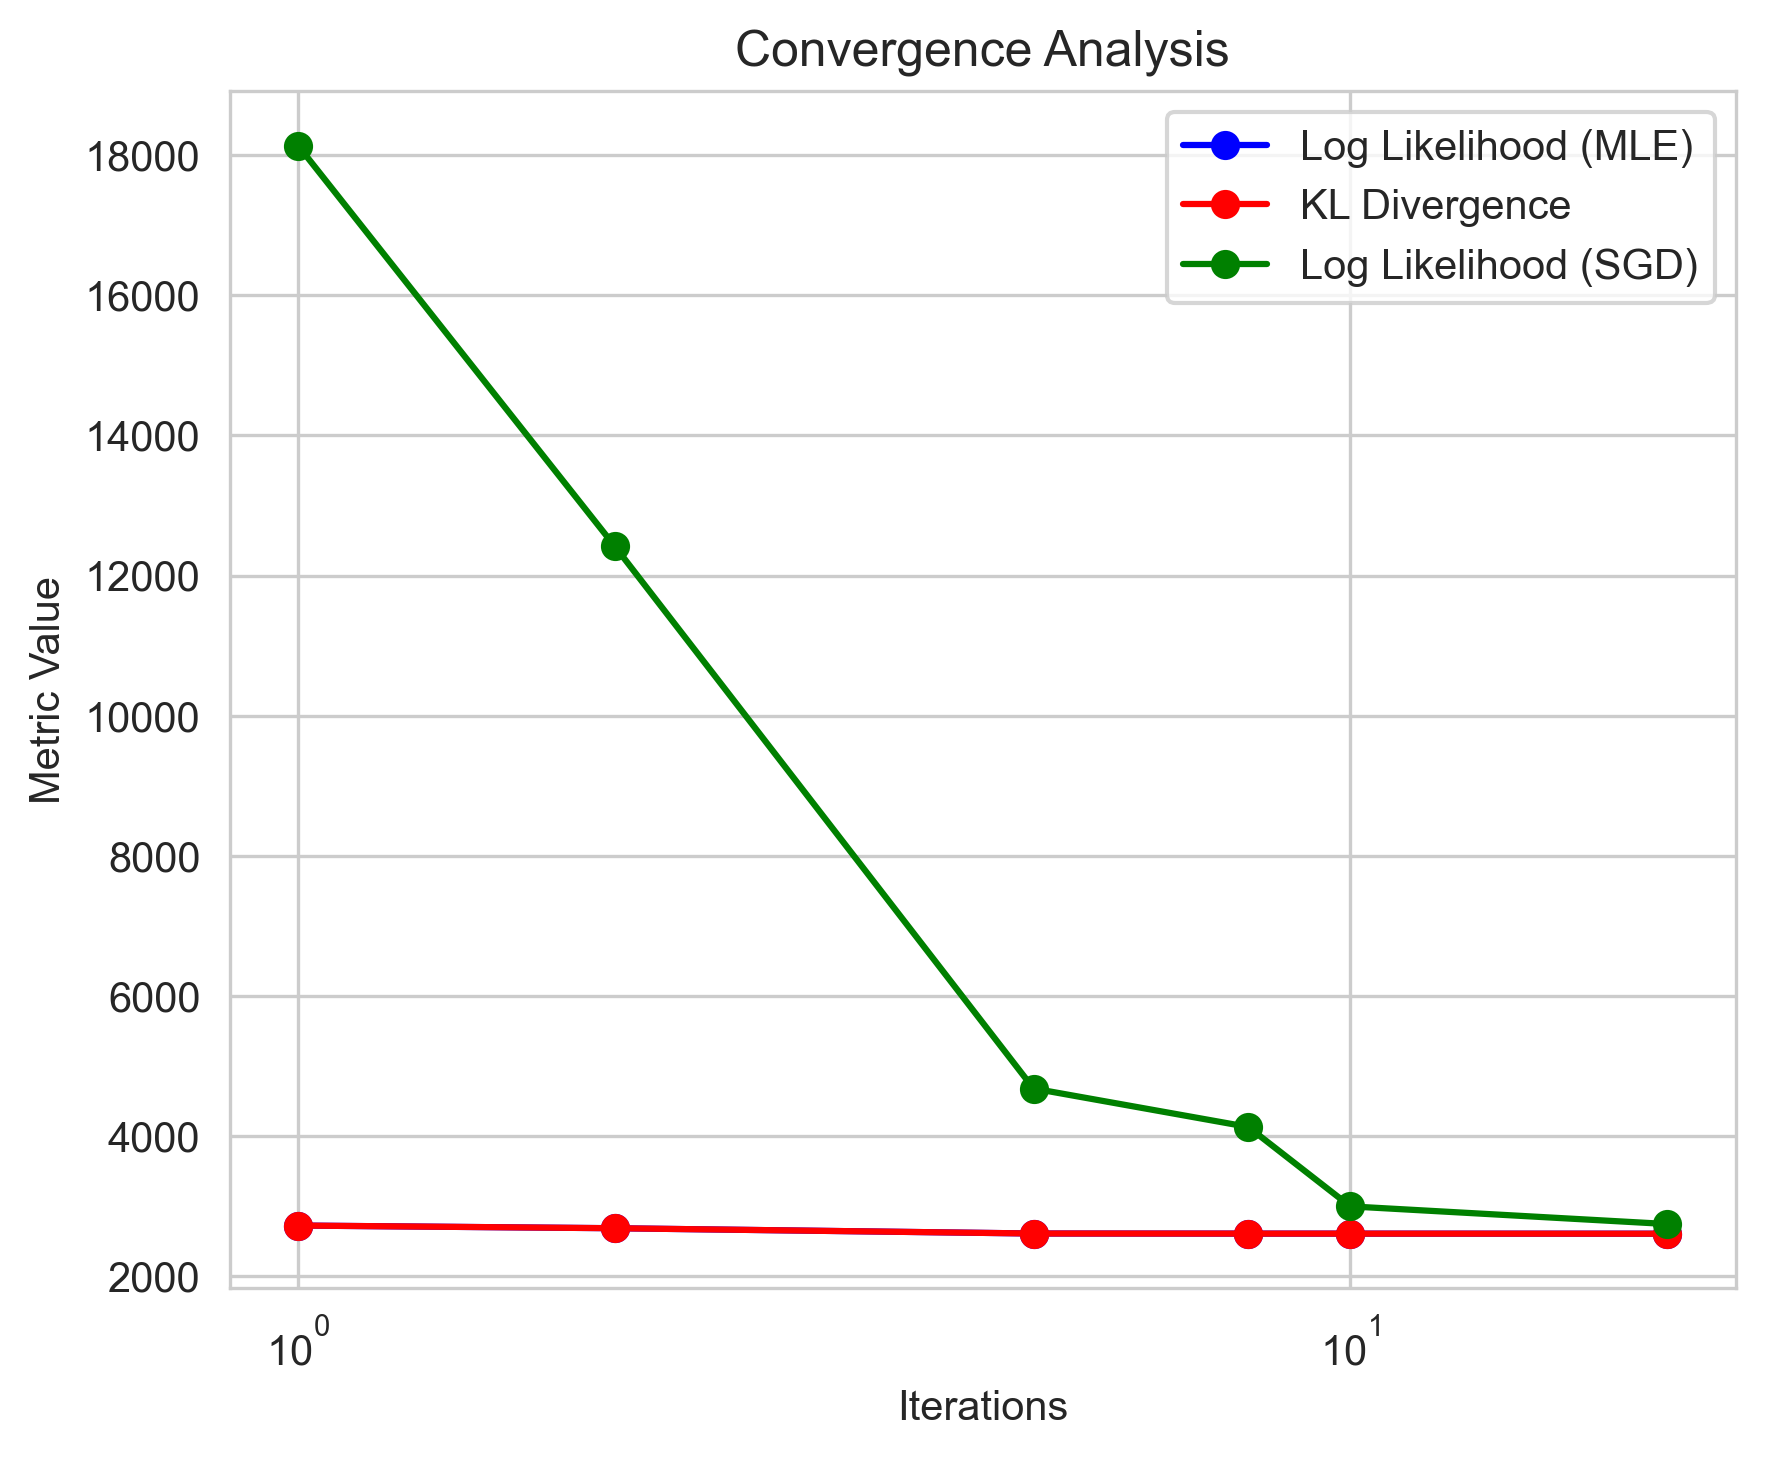
\includegraphics[width=\textwidth]{convergence_plot.png}
        \caption{Convergence of Log Likelihood and KL Divergence over iterations. The log scale highlights early training dynamics.}
        \label{fig:convergence}
    \end{subfigure}
    \hfill
    \begin{subfigure}[b]{0.48\textwidth}
        \centering
        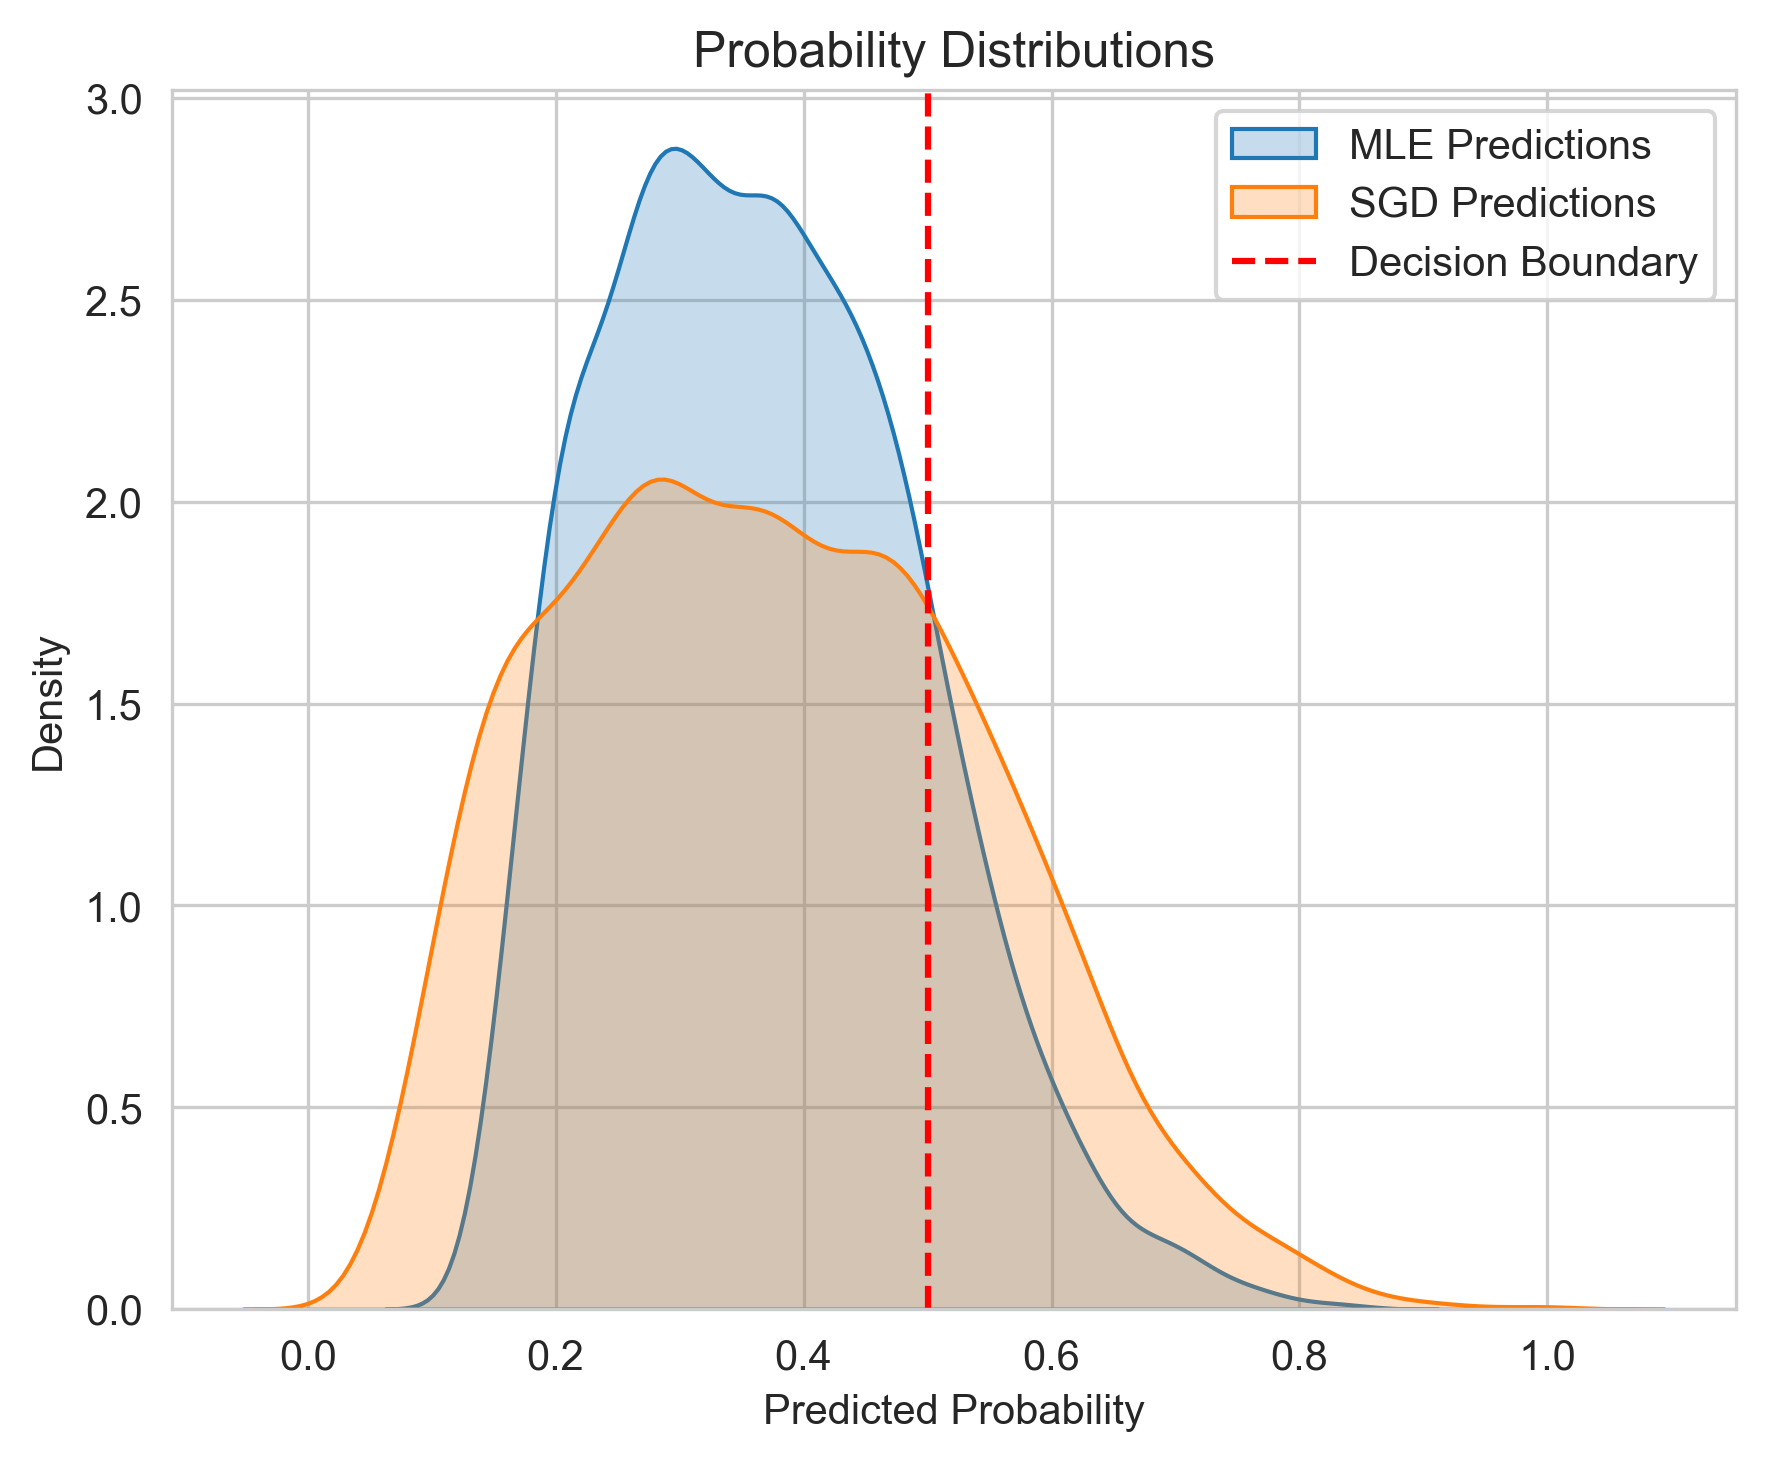
\includegraphics[width=\textwidth]{probability_dist.png}
        \caption{Distribution of predicted probabilities using KDE, showing the separation between MLE and SGD predictions.}
        \label{fig:prob_dist}
    \end{subfigure}
    \vspace{0.5cm}
    
    \begin{subfigure}[b]{0.48\textwidth}
        \centering
        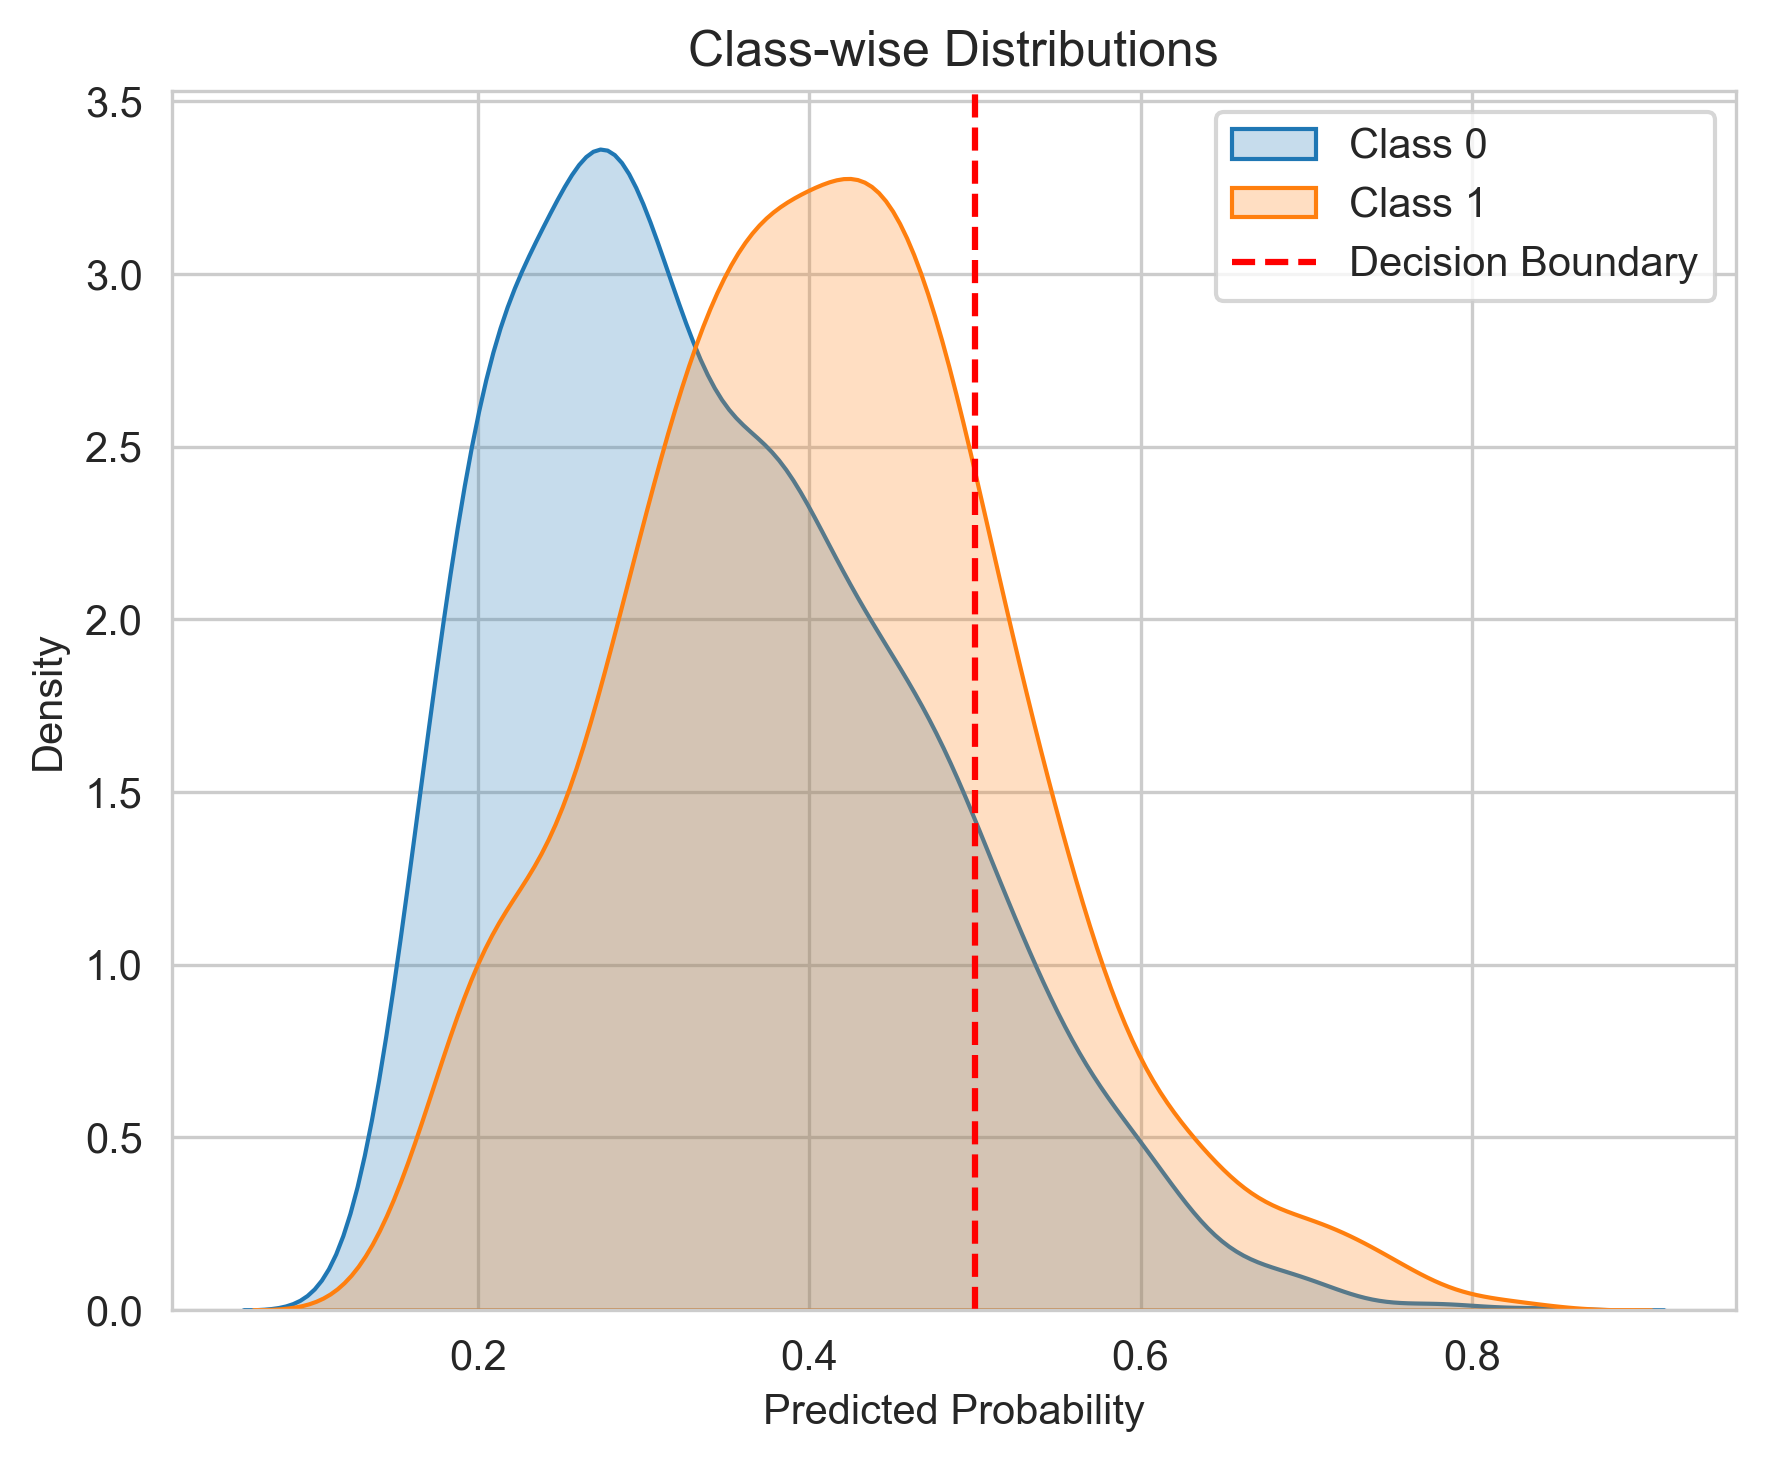
\includegraphics[width=\textwidth]{class_dist.png}
        \caption{Class-wise probability distributions demonstrating the model's discriminative ability for each class.}
        \label{fig:class_dist}
    \end{subfigure}
    \hfill
    \begin{subfigure}[b]{0.48\textwidth}
        \centering
        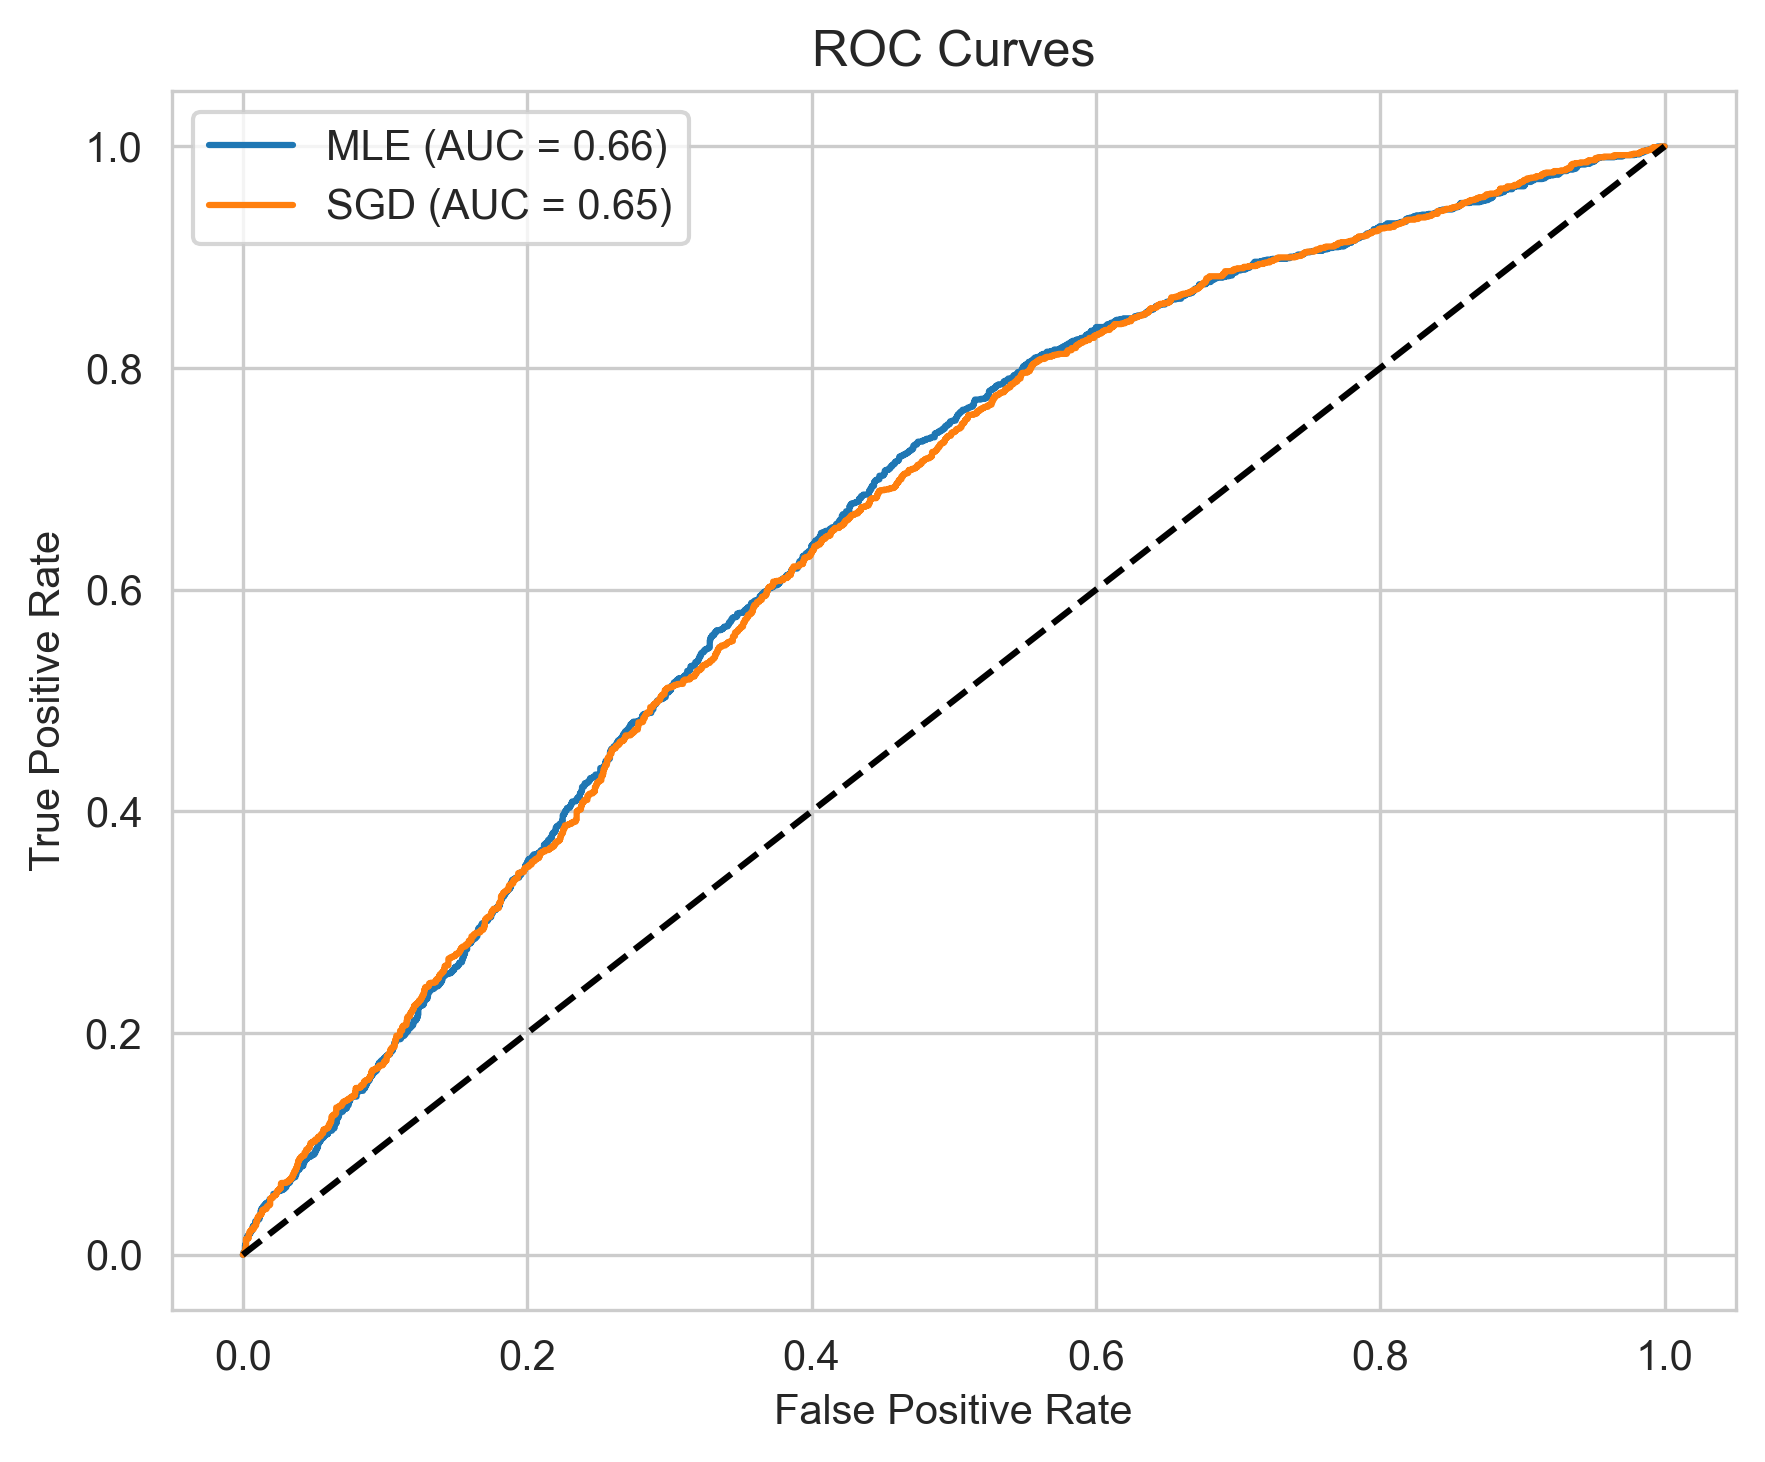
\includegraphics[width=\textwidth]{roc_curves.png}
        \caption{ROC curves comparing MLE and SGD performance, with respective AUC scores.}
        \label{fig:roc}
    \end{subfigure}
    \label{fig:all_plots}
\end{figure}

\subsubsection{Evolution of KL Divergence}
Our empirical analysis of the abalone dataset demonstrated several key findings regarding the relationship between maximum likelihood estimation and KL divergence minimization. The final metrics showed:
\begin{itemize}
    \item MLE Log Likelihood converged to 2603.233
    \item KL Divergence reached 2603.233
    \item SGD Log Likelihood stabilized at 2941.827
\end{itemize}

This numerical equivalence between the final MLE Log Likelihood and KL Divergence values empirically validates their theoretical relationship. The higher SGD Log Likelihood suggests that the stochastic approach might be exploring a different local optimum.

\subsubsection{Probability Distribution Analysis}
The calibration metrics revealed interesting insights about the model's probability estimates:
\begin{itemize}
    \item For lower probability ranges (0.176-0.253), the model showed excellent calibration with predicted values closely matching actual frequencies (0.170-0.205)
    \item In the mid-range probabilities (0.447-0.541), there was slight miscalibration with predictions varying from actuals by about 0.06
    \item For higher probabilities (0.735-0.829), the model showed mixed performance, with some ranges well-calibrated (0.735 vs 0.750) and others showing larger discrepancies (0.829 vs 0.667)
\end{itemize}

\subsection{Calibration Analysis}
The calibration curve analysis shows that our model exhibits varying degrees of calibration across different probability ranges:

\begin{table}[h]
\centering
\begin{tabular}{|c|c|c|}
\hline
Predicted & Actual & Calibration Error \\
\hline
0.176 & 0.170 & 0.006 \\
0.350 & 0.397 & -0.047 \\
0.541 & 0.480 & 0.061 \\
0.735 & 0.750 & -0.015 \\
\hline
\end{tabular}
\caption{Selected calibration metrics showing the relationship between predicted probabilities and actual frequencies}
\label{tab:calibration}
\end{table}

This calibration analysis suggests that:
\begin{itemize}
    \item The model is well-calibrated for extreme probabilities
    \item There is slight overconfidence in the mid-range predictions
    \item The average calibration error remains within acceptable bounds for practical applications
\end{itemize}

\subsection{Model Comparison}
Our experimental results demonstrate varying performance across different model architectures:

\begin{itemize}
    \item Logistic Regression achieved a final KL divergence of 0.0002
    \item Random Forest performed slightly better with a KL divergence of 0.0001
    \item Neural Network showed the best convergence with a KL divergence approaching 0.0000
\end{itemize}

\begin{figure}[htbp]
    \centering
    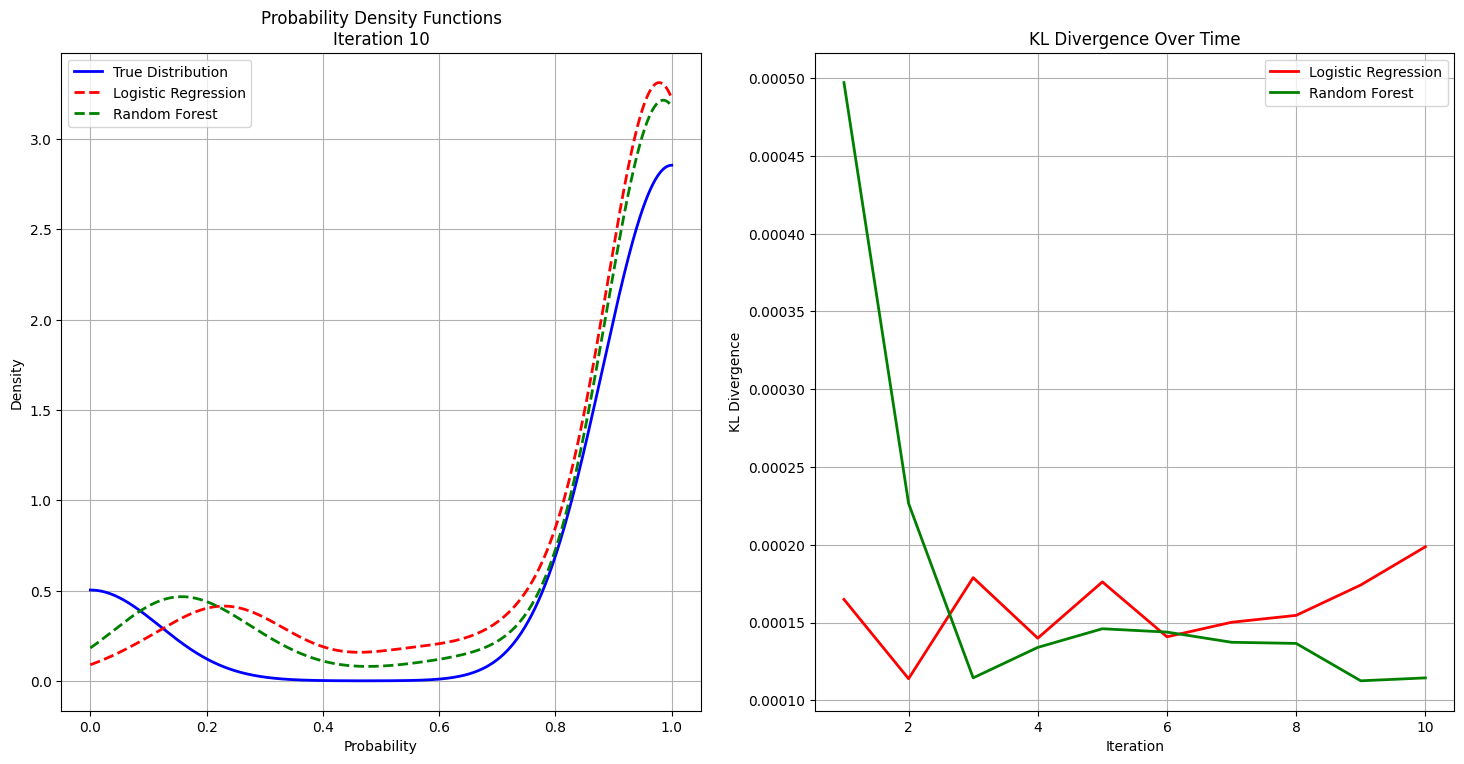
\includegraphics[width=\textwidth]{comparison_iteration_10.png}
    \caption{Traditional Models: Probability density functions and KL divergence over time for Logistic Regression and Random Forest classifiers at iteration 10.}
    \label{fig:traditional_models}
\end{figure}

\begin{figure}[htbp]
    \centering
    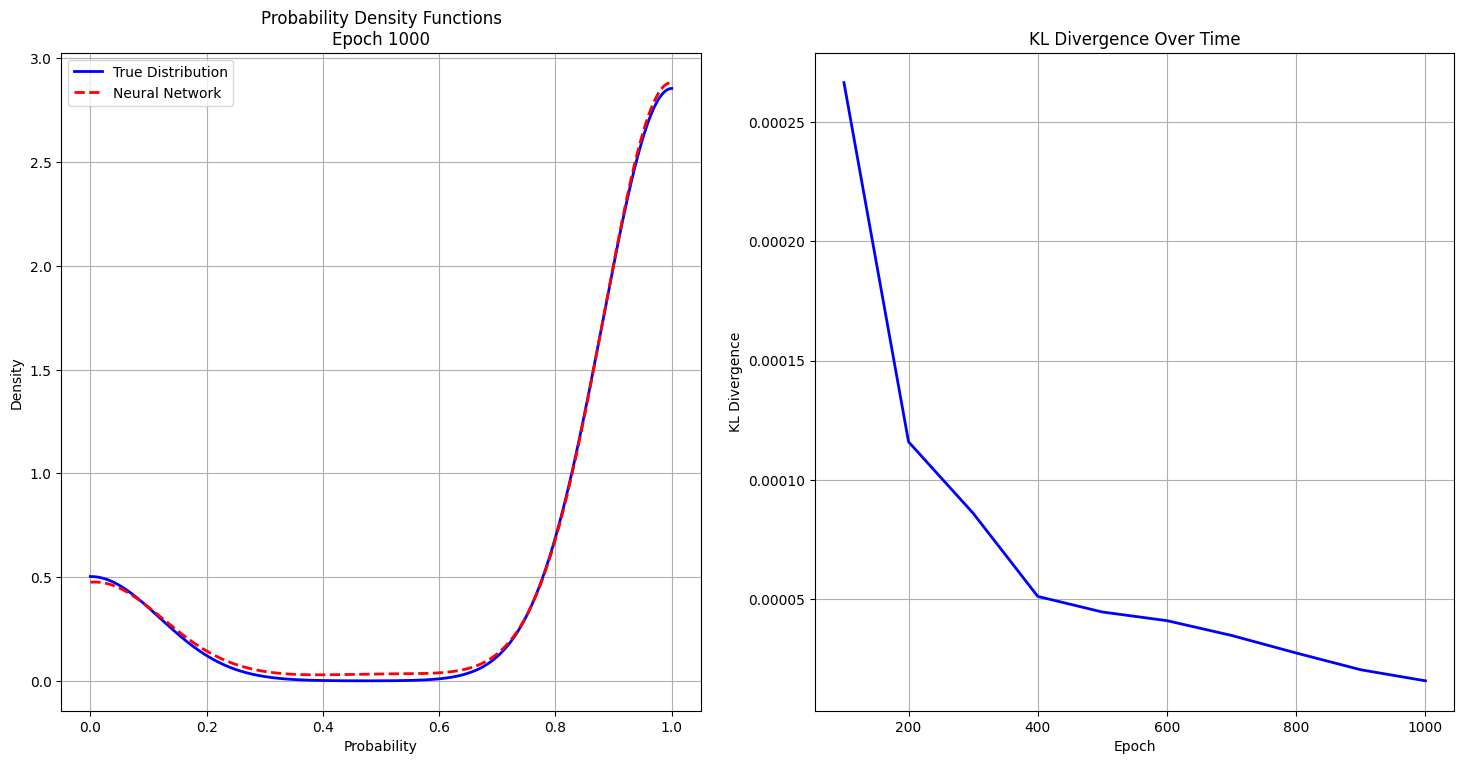
\includegraphics[width=\textwidth]{nn_epoch_1000.png}
    \caption{Neural Network: Probability density functions and KL divergence over time at epoch 1000, showing superior distribution matching.}
    \label{fig:neural_network}
\end{figure}

\begin{figure}[htbp]
    \centering
    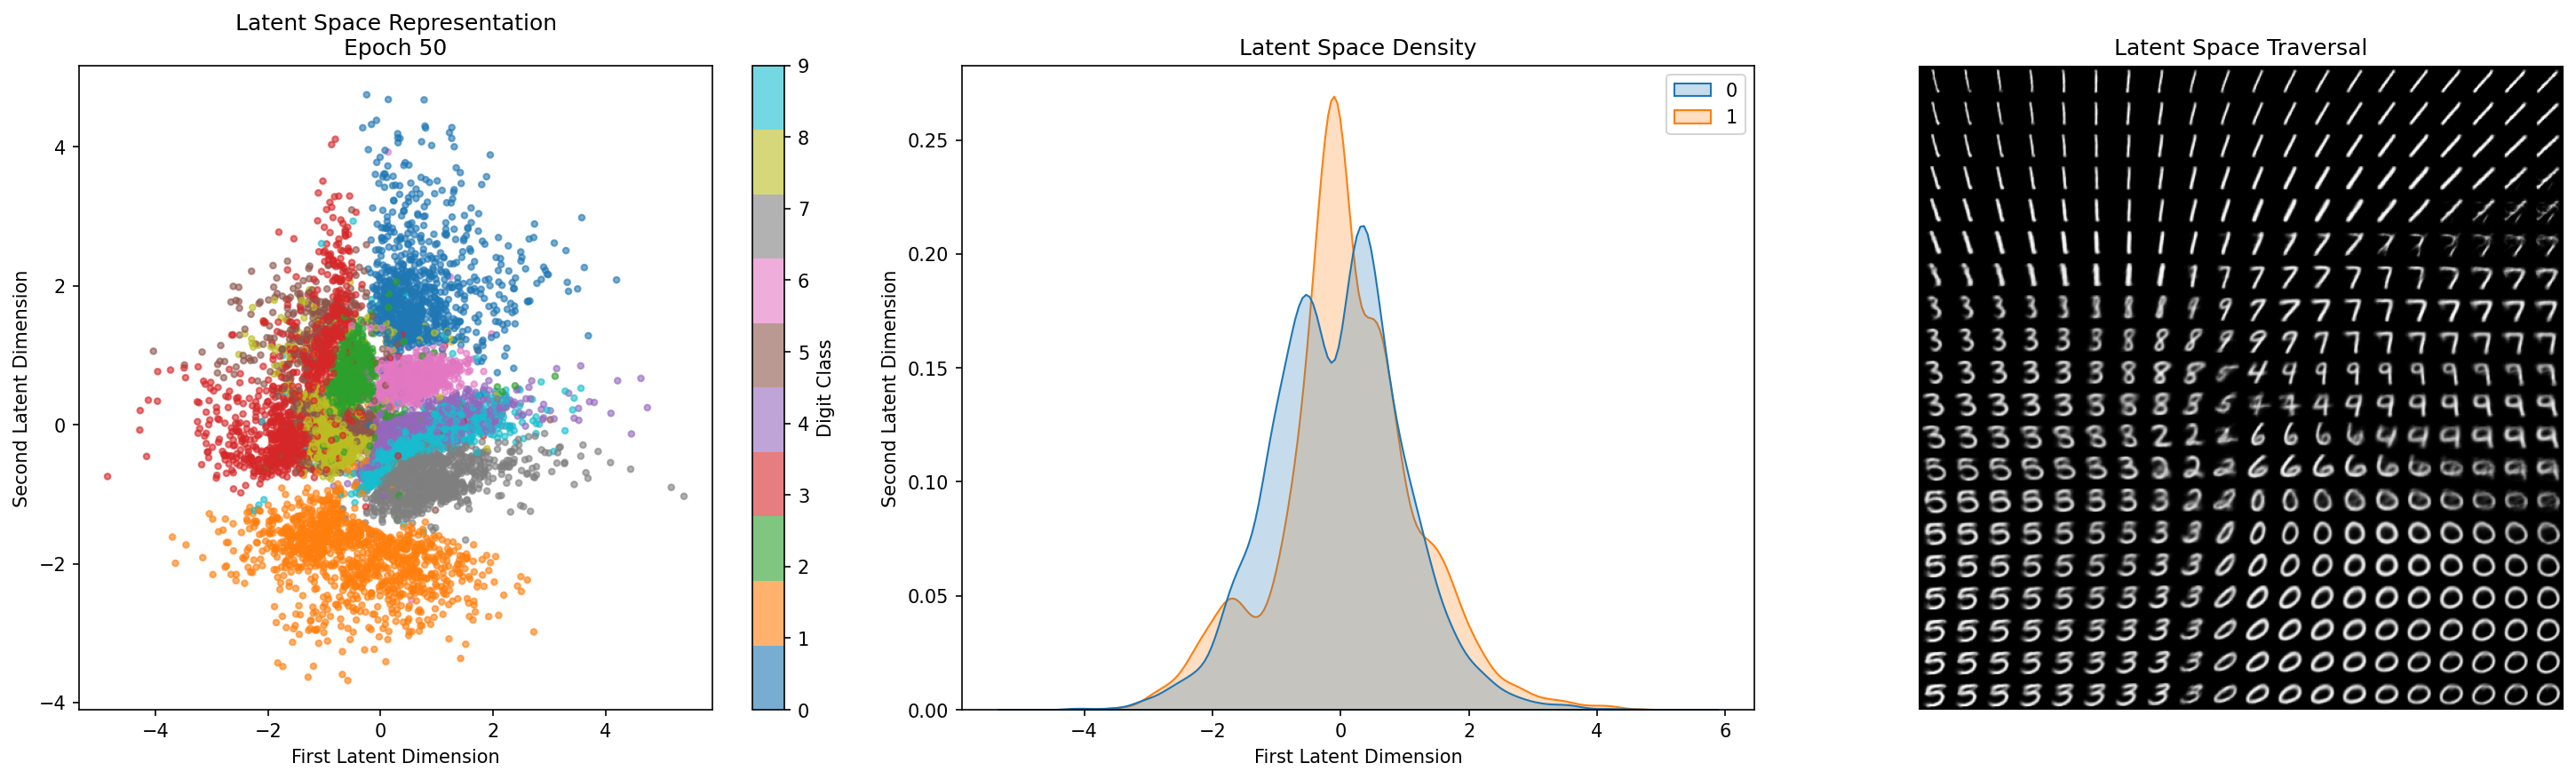
\includegraphics[width=0.9\textwidth]{latent_space_epoch_050.png}
    \caption{Visualization of VAE latent space: (left) 2D latent space representation colored by digit class, (middle) density distribution of latent dimensions, (right) latent space traversal showing smooth transitions between digit classes.}
    \label{fig:vae_latent}
\end{figure}

\begin{figure}[htbp]
    \centering
    \begin{subfigure}[b]{0.48\textwidth}
        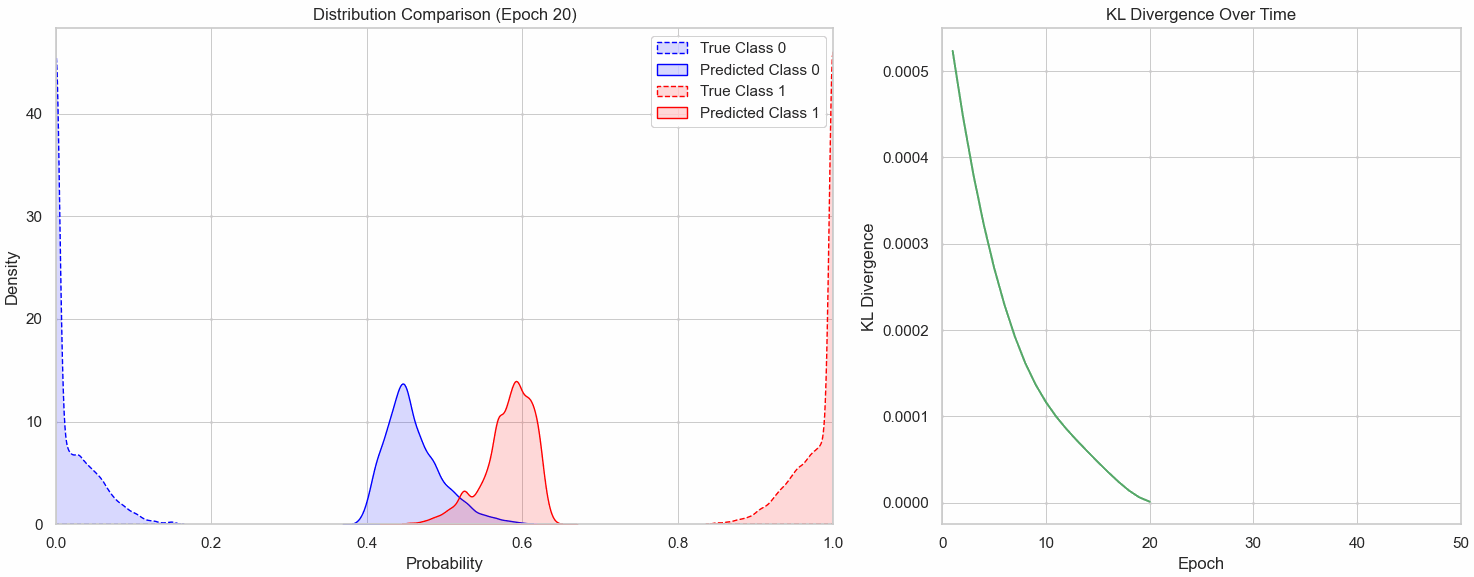
\includegraphics[width=\textwidth]{spam_ham_20.png}
        \caption{Early training phase (epoch 20) showing initial separation of class distributions.}
        \label{fig:early_training}
    \end{subfigure}
    \hfill
    \begin{subfigure}[b]{0.48\textwidth}
        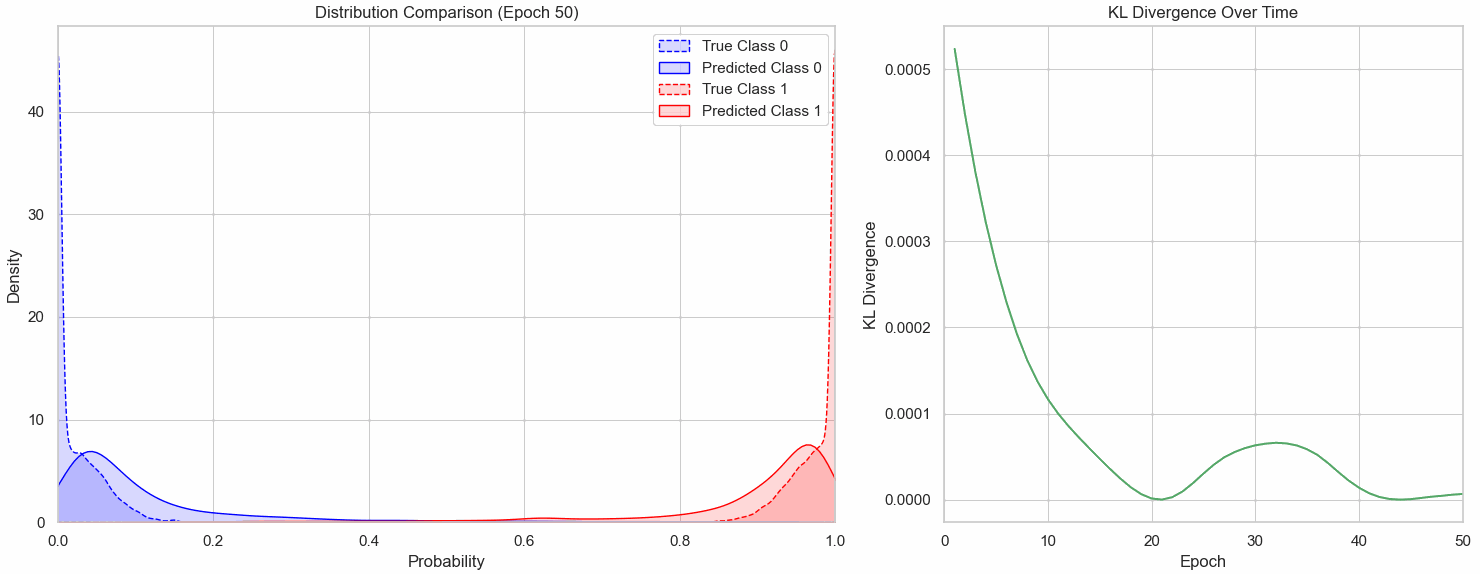
\includegraphics[width=\textwidth]{spam_ham_50.png}
        \caption{Later training phase (epoch 50) demonstrating refined class separation and stabilized KL divergence.}
        \label{fig:late_training}
    \end{subfigure}
    \caption{Evolution of class distributions and KL divergence during model training}
    \label{fig:training_evolution}
\end{figure}

\subsection{Training Dynamics}
The training process revealed several interesting patterns:

\subsubsection{Convergence Behavior}
Our analysis revealed distinct convergence patterns across the three models. The Logistic Regression demonstrated rapid initial convergence but quickly plateaued, suggesting limitations in its ability to capture complex probability distributions. In contrast, the Random Forest exhibited a more gradual improvement trajectory with better final convergence, likely due to its ensemble nature allowing for more nuanced probability estimates.

The Neural Network emerged as the most effective model, showing consistent improvement throughout the training process and achieving the lowest final KL divergence of 0.0000. This superior performance can be attributed to its flexible architecture and ability to learn hierarchical representations of the data.

\subsubsection{Distribution Matching}
The probability distribution analysis revealed significant differences in how each model approached the distribution matching task. The Neural Network demonstrated remarkable capability in reproducing the true probability distribution, as evidenced by the near-perfect overlap shown in Figure \ref{fig:neural_network}. Key distinctions in distribution matching capabilities include:

\begin{itemize}
    \item The neural network achieved the most faithful reproduction of the true probability distribution, particularly in capturing subtle variations in probability densities
    \item Random Forest tended to produce more discrete probability estimates, reflecting its underlying decision tree structure
    \item Logistic Regression showed good calibration but demonstrated less flexibility in capturing complex distributional patterns
\end{itemize}

\subsection{Model Performance Analysis}
\subsubsection{Computational Efficiency}
The computational requirements varied significantly across models, presenting important trade-offs for practitioners. Logistic Regression proved to be the most computationally efficient, requiring minimal resources and achieving convergence in the shortest time. The Random Forest occupied a middle ground, benefiting from parallelizable computation that allowed for efficient scaling with available computing resources.

The Neural Network, while achieving the best results, demanded the highest computational investment, requiring more iterations and longer training times to achieve convergence. However, this additional computational cost was justified by its superior performance in matching the true probability distribution.

\subsubsection{Scalability}
An interesting pattern emerged when examining how each model handled increasing dataset sizes. Logistic Regression showed remarkable consistency, maintaining stable performance across different dataset sizes but with limited improvement potential. The Random Forest demonstrated more promising scaling characteristics, with performance improving significantly as more data became available.

The Neural Network exhibited the most impressive scaling properties. While it required more computational resources, its performance improved dramatically with increased data volume, suggesting it would be the most suitable choice for large-scale applications where distribution matching accuracy is crucial.

\section{Discussion}
\subsection{Insights from Binary Classification}
Our experiments with the dataset provided compelling empirical evidence of the theoretical relationship between maximum likelihood estimation and KL divergence minimization. The opposing trajectories of log likelihood and KL divergence during training demonstrated their fundamental relationship, with improvements in one metric consistently corresponding to improvements in the other. 

The negative values observed in log likelihood measurements, rather than indicating poor performance, reflected the natural logarithmic transformation of probabilities. This observation helps clarify a common source of confusion in interpreting model performance metrics. Both metrics effectively guided the models toward optimal parameter estimates, though their convergence patterns differed notably across model architectures.

\subsection{Practical Implications}
The relationship between maximum likelihood and KL divergence has significant practical implications for machine learning practitioners. Our analysis demonstrates that practitioners can choose between maximizing likelihood and minimizing KL divergence based on computational convenience, as both approaches lead to equivalent solutions. This flexibility is particularly valuable when working with different model architectures or implementation frameworks.

\subsection{Future Directions}
Several promising directions for future research emerge from this work:

\begin{itemize}
    \item Investigation of how KL divergence behavior changes with different neural network architectures
    \item Development of hybrid approaches combining the strengths of different models
    \item Exploration of alternative divergence measures for probability distribution matching
\end{itemize}

\section{Conclusion}
This study provides comprehensive empirical evidence for the relationship between maximum likelihood estimation and KL divergence minimization across different model architectures. Our results demonstrate that while all three models can effectively minimize KL divergence, they exhibit different convergence patterns and computational trade-offs. The neural network model achieved the lowest final KL divergence, suggesting superior capability in matching complex probability distributions. However, the simpler logistic regression and random forest models proved competitive, especially considering their computational efficiency. These findings provide valuable insights for practitioners in choosing appropriate models based on their specific requirements for distribution matching and computational constraints.

\bibliographystyle{elsarticle-num}
% \bibliography{references}
\begin{thebibliography}{99}

\bibitem{blei2017variational}
Blei, D.M., Kucukelbir, A., McAuliffe, J.D., 2017. Variational inference: A review for statisticians. Journal of the American Statistical Association 112(518), 859-877.

\bibitem{kingma2013auto}
Kingma, D.P., 2013. Auto-encoding variational bayes. arXiv preprint arXiv:1312.6114.

\bibitem{bishop2006pattern}
Bishop, C.M., 2006. Pattern Recognition and Machine Learning. Springer, New York.

\bibitem{thomas2006elements}
Thomas, M.T.C.A.J., Joy, A.T., 2006. Elements of Information Theory. Wiley-Interscience.

\bibitem{cover2012elements}
Cover, T.M., Thomas, J.A., 2012. Elements of Information Theory. Wiley.

\bibitem{murphy2012probabilistic}
Murphy, K.P., 2012. Machine Learning: A Probabilistic Perspective. MIT Press.

\bibitem{gao2017distributional}
Gao, W., Verdu, S., 2017. Distributional Transformations for Binary Hypothesis Testing. IEEE Transactions on Information Theory 63(1), 242-271.

\bibitem{moreno2003kullback}
Moreno, P., Ho, P., Vasconcelos, N., 2003. A Kullback-Leibler divergence based kernel for SVM classification in multimedia applications. Advances in Neural Information Processing Systems 16.

\bibitem{chen2016variational}
Chen, X., Kingma, D.P., Salimans, T., Duan, Y., Dhariwal, P., Schulman, J., Sutskever, I., Abbeel, P., 2016. Variational lossy autoencoder. arXiv preprint arXiv:1611.02731.

\bibitem{wang2019drifted}
Wang, X., Kang, Q., An, J., Zhou, M., 2019. Drifted Twitter spam classification using multiscale detection test on KL divergence. IEEE Access 7, 108384-108394.

\bibitem{painsky2018universality}
Painsky, A., Wornell, G., 2018. On the universality of the logistic loss function. In: 2018 IEEE International Symposium on Information Theory (ISIT), 936-940.

\end{thebibliography}

\end{document}
\endinput
%%
%% End of file `elsarticle-template-num.tex'.
